\section{Evaluation}
\label{sec:eval}

In order to evaluate Multisurf, we ask the following questions:

\begin{itemize}
\item How much does it cost to use Multisurf in terms of performance?
\item How accurately does Multisurf classify ``safe'' and ``unsafe'' sites?
\end{itemize}

We answer these questions by measuring the latency of our system, as well as analyzing the results of running our system using different comparison algorithms.

Our measurements are taken using the Alexa Top 100~\cite{alexa} websites as our dataset.  All of our experiments were performed using a laptop with a 2 GHz Intel Core 2 Duo processor.  

\subsection{Latency} 
For each web page, we measure the latency from the client; this is measuring the time for the client to make her own request, the time for the client to ask her peer to make the same request, and the time for the peer to make the request and return her response to the client.  Using the Alexa Top 50 websites, we measure the latency 50 times and take the average.  This is repeated for the four different comparison algorithms that Multisurf can use, as well as a base line measurement of the latency solely for the client to make a request.  The results are shown in Figure~\ref{fig:latency}.

\begin{figure}[htb]
\label{fig:latency}
\begin{center}
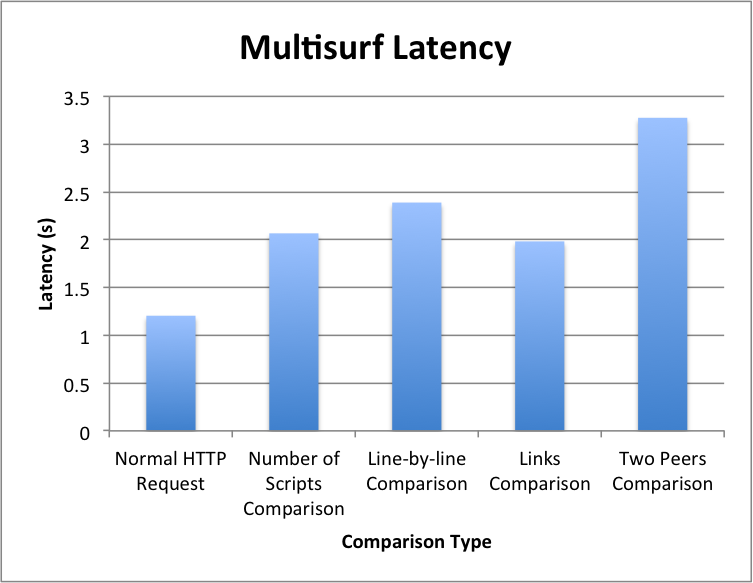
\includegraphics[width=\linewidth]{latency}
\caption{This is a figure.}
\end{center}
\end{figure}

The latency of the different methods in comparison to one another are what was expected.  When the client sends just her own request, without interacting with her peer, she has the lowest latency.  On the other hand, the highest latency occurs when the client uses two peers to determine if a site is safe; she must send her own request in addition to asking two peers to send their requests.  Overall, the latencies were relatively similar and the additional time it took to use Multisurf does not outweigh the benefits.  

\subsection{Accuracy}
We measure accuracy in terms of the number of websites that are classified as ``safe'' and ``unsafe.''  Once the client recieves her own response as well as the response her peer sends, both responses go through a comparison, and are then placed in one of six categories:

\begin{enumerate}
\item ``Safe''
\item ``Unsafe''
\item Identical responses, but no content to compare
\item Different responses, but no content to compare
\item HTTPS-Only
\item Error
\end{enumerate}

In determining accuracy, we only consider the first two categories.  A ``safe'' site is one that was determined by the comparison algorithm to not have a man in the middle attack; an ``unsafe'' site is one that was determined by the comparison algorithm to possibly have a man in the middle attack.  For our measurements, we assume that there were no man in the middle attacks and 100\% accuracy would be no ``unsafe'' sites.  We calculated the accuracy for our four different comparison methods: comparing the number of scripts, comparing line by line, comparing the links, and comparing line by line with two peers.

\subsubsection{Number of Scripts}
Figure~\ref{fig:scripts} shows the results of using Multisurf with the comparison algorithm that compares the number of scripts in each response.  The accuracy is 34.39\%.  This shows that there are a significant number of websites that send a different number of scripts in each response.

\begin{figure}[htb]
\label{fig:scripts}
\begin{center}
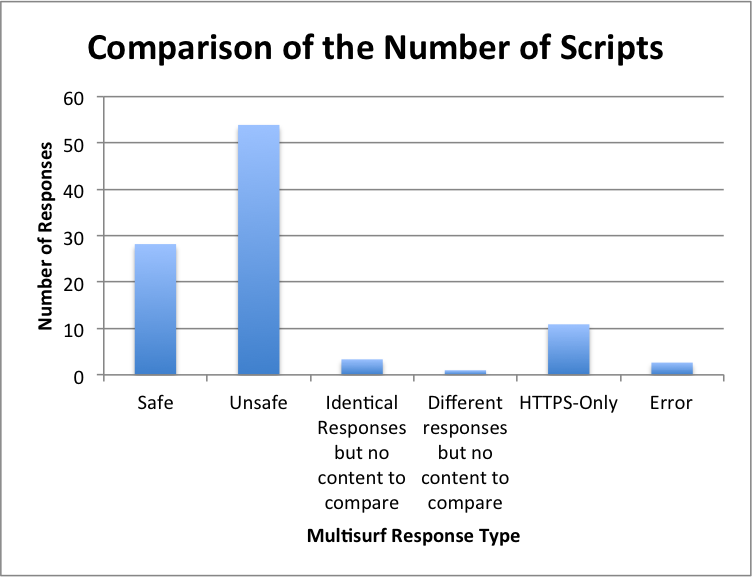
\includegraphics[width=\linewidth]{scripts}
\caption{This is a figure.}
\end{center}
\end{figure}

\subsubsection{Line by Line}
When comparing the responses line by line, Multisurf exhibited only 8.72\% accuracy.  The amount of dynamic web content on the Internet is a large factor in the low accuracy rate of this method.  The results are shown in Figure~\ref{fig:lines}.

\begin{figure}[htb]
\label{fig:lines}
\begin{center}
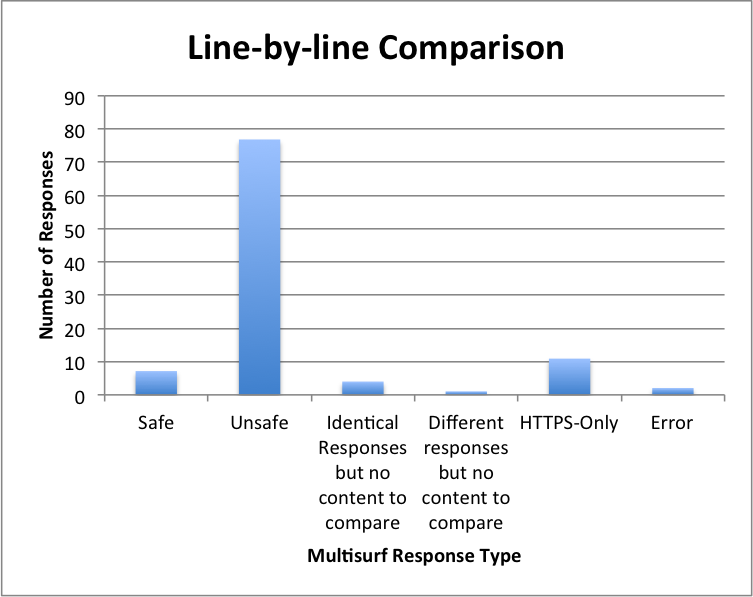
\includegraphics[width=\linewidth]{lines}
\caption{This is a figure.}
\end{center}
\end{figure}

\subsubsection{Links}
A possible man in the middle attack is to inject or change a URL in the response to take the client to a malicious site.  The Multisurf response types for comparing which links are in each response are shown in Figure~\ref{fig:links}; this method has an accuracy of 46.16\%. 

\begin{figure}[htb]
\label{fig:links}
\begin{center}
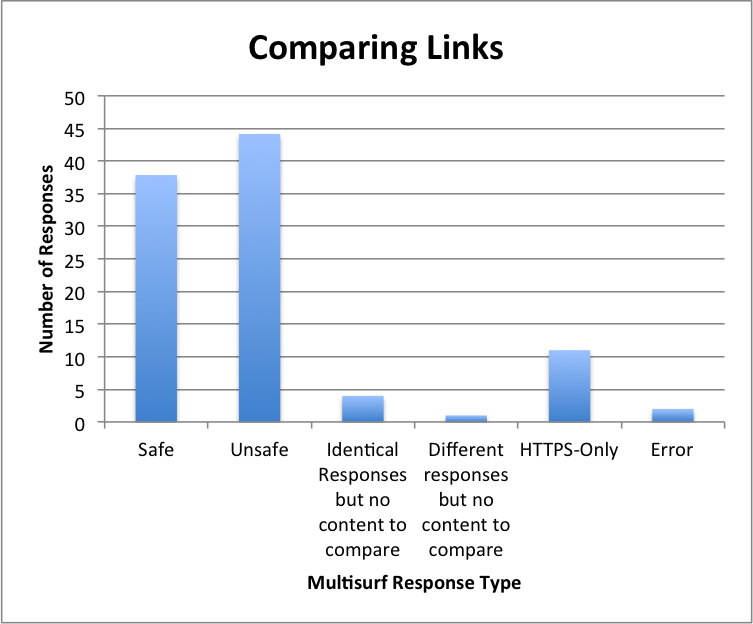
\includegraphics[width=\linewidth]{links}
\caption{This is a figure.}
\end{center}
\end{figure}

\subsubsection{Line by Line with Two Peers}
The accuracy rates for the three comparison methods above are relatively low; this can be improved by adding a second peer.  In this case, we check to see if the response of the client is different from either of the peers' responses.  If the peers' responses are the same (as measured line by line) and the client's response is different (as measured line by line), then the site is classified as ``unsafe.''  Otherwise, the site is deemed ``safe.''  The accuracy for this method is 100\% and can be seen in Figure~\ref{fig:twopeers}.

\begin{figure}[htb]
\label{fig:peers}
\begin{center}
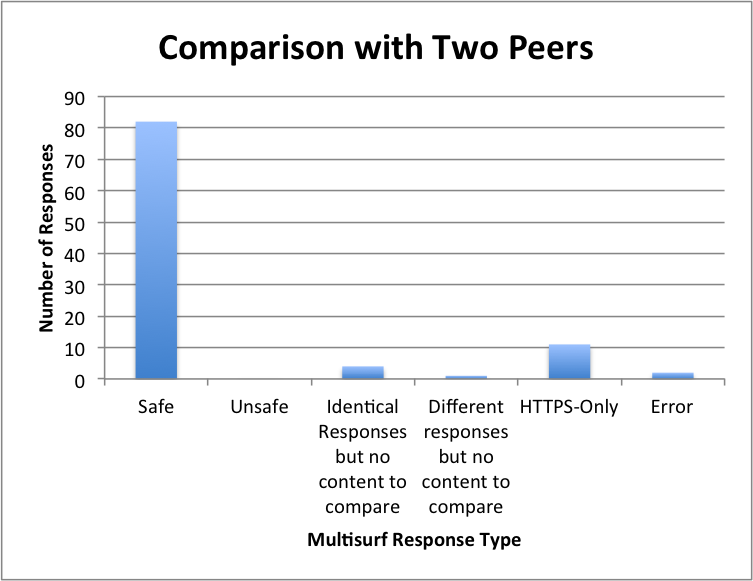
\includegraphics[width=\linewidth]{twopeers}
\caption{This is a figure.}
\end{center}
\end{figure}
